
\begin{figure}[t]
\centering

\begin{subfigure}[t]{\columnwidth}
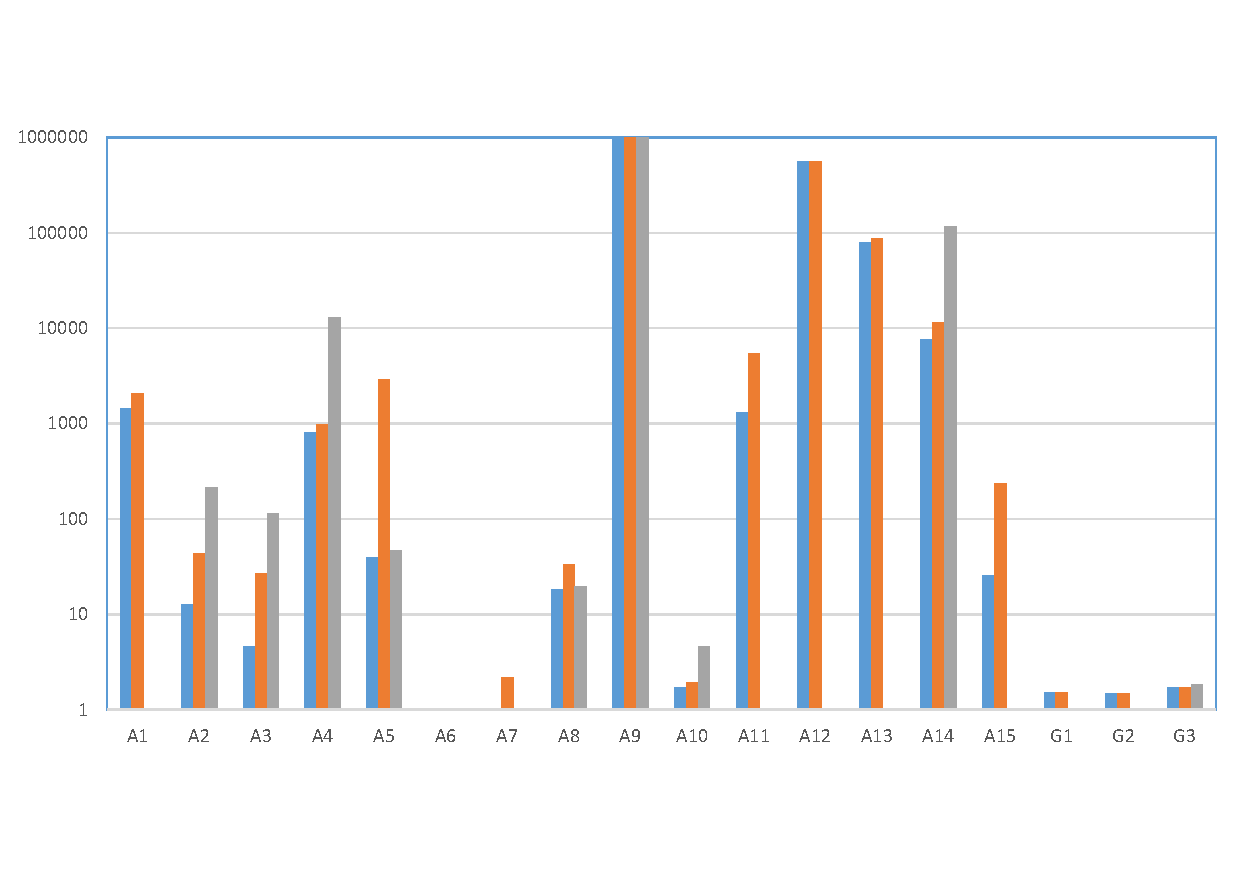
\includegraphics[clip, trim=0.8cm 2cm 0.9cm 2.15cm,
width=\columnwidth]{graphs/data_red.pdf}
\caption{Processed data reduction}
\label{fig:data_red}
\end{subfigure}
~
\begin{subfigure}[t]{\columnwidth}
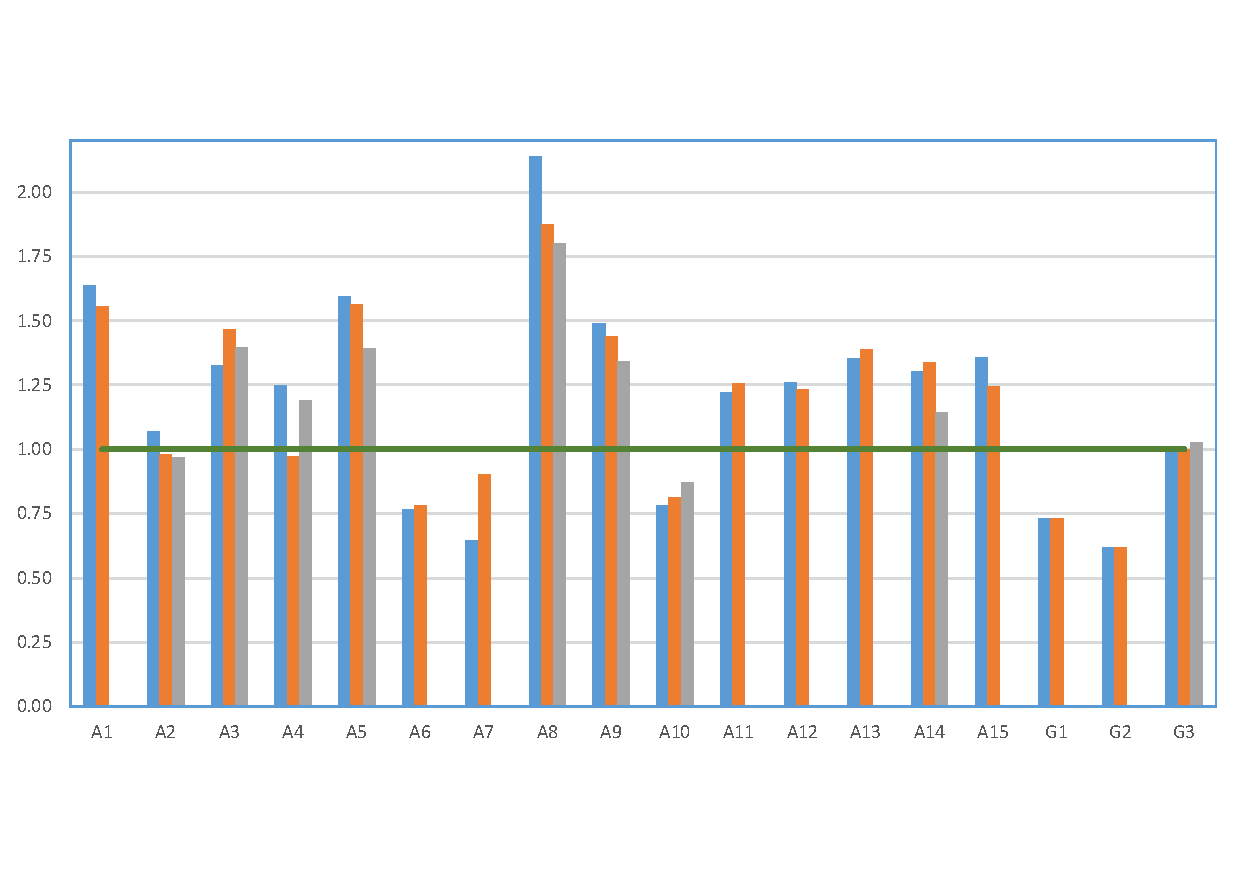
\includegraphics[clip, trim=0.8cm 2cm 0.9cm 2cm,
width=\columnwidth]{graphs/processing_red.pdf}
\caption{Processing time reduction}
\label{fig:processing_red}
\end{subfigure}
~
\begin{subfigure}[t]{\columnwidth}
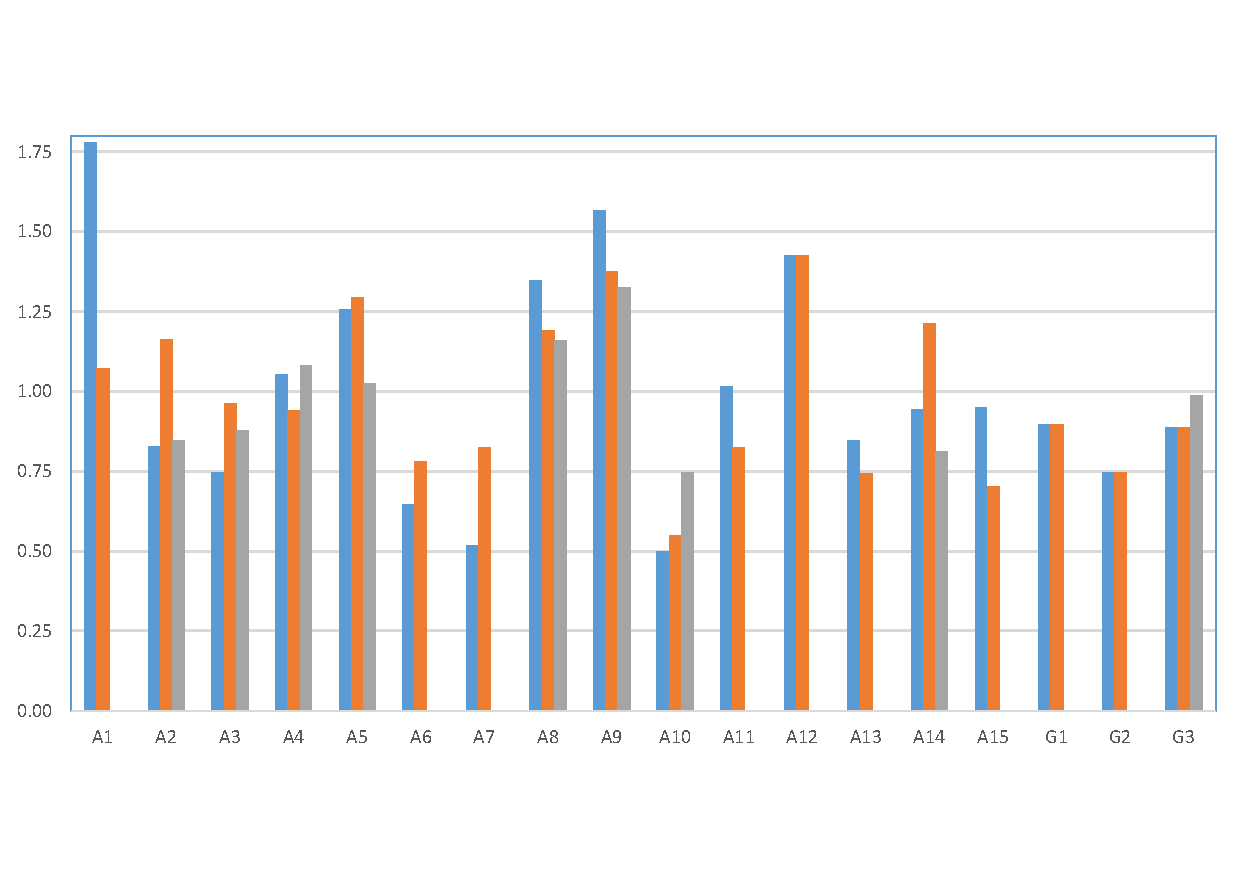
\includegraphics[clip, trim=0.8cm 1.5cm 0.9cm 1cm,
width=\columnwidth]{graphs/latency_red.pdf}
\caption{Latency reduction}
\label{fig:latency_red}
\end{subfigure}

\caption{Reduction ratios of the processed data, processing time and latency
when using abstract filters divided by the corresponding baseline measures.}
\end{figure}





\section{Evaluation}

We tested our approach on 2 workloads:
i) patterns over telemetry events collected within a 2 hours interval by the
Asimov system, and 
ii) repository analytics over the Github dataset consisting of events collected
between 2011 and 2016.



We assess the benefits provided by our approach in terms of the ratio of
selected events vs input events, the time it takes to complete the query
(latency), and the total execution time across the processing nodes of the
cluster.


We further break down the {\em baseline} execution of a query into the time it
takes to 
i) read and sort the data, and 
ii) perform the reduction step.
On the other hand for our approach we look at the time it takes to 
i) read the data and build the symbolic state associated with each transition,
ii) reduce the symbolic state associated to each transition down to an abstract
filter for the entire query and broadcast it back to every mapper,
iii) filter the input events based on the abstract filter, and
iv) perform the reduction step over the remaining events. 


In addition we conduct experiments to highlight the filtering potential of
different join predicates, as well as their sensitivity wrt.\ the amount of
state dedicated to their symbolic representation.



\subsection{Processed data reduction}

In order to establish the raw potential of our approach we look at the amount of
data that is discarded by the abstract filters that we build.
We note that the baseline consists of events whose type matches the event type
of a transition in the query.


\subsection{Total processing time reduction}


\subsection{Latency reduction}

\subsection{Symbolic state size vs filtering ratio tradeoff}